\section{ОСОБЕННОСТИ РЕАЛИЗАЦИИ ОБРАЗОВАТЕЛЬНОЙ ПЛАТФОРМЫ}
\addcontentsline{toc}{section}{Особенности  реализации образовательной платформы}

В данном разделе описаны детали реализации приложения, а также приведены результаты его тестирования.
В ходе работы над проектом необходимо было реализовать модульные компоненты, которые позволили
бы в дальнейшем минимизировать трудозатраты на доработки и расширение системы.

\subsection{Структура приложения}

После анализа возможных вариантов реализации приложения, была выбрана многоуровневая архитектура,
каждый уровень отвечает за свою логическую часть.

В стандарте IEEE 1471 дается следующее определение: «Архитектура – это базовая организация
системы, которая описывает связи между компонентами этой системы (и внешней средой),
а также определяет принципы её проектирования и развития». Однако многие другие определения
архитектуры признают не только структурные элементы, но и их композиции, а также интерфейсы
и другие соединительные звенья.

Многоуровневая архитектура – является одной из самых известных архитектур, в которой
каждый слой выполняет определенную функцию. В зависимости от ваших нужд вы можете
реализовать любое количество уровней, но слишком большое их количество приведет к
чрезмерному усложнению системы. Часто выделяют три основных уровня: уровень представления,
уровень логики и уровень данных.

Слою не обязательно знать, что делают его соседи. Здесь проявляется такое свойство как
разделение ответственности. Если все три слоя являются закрытыми, то запрос пользователя
к верхнему уровню инициирует цепочку обращений с верхнего уровня до самого нижнего.
В этом случае уровень представления отвечает за пользовательский интерфейс и отображение
данных для пользователя и ничего не знает о существовании физического хранилища данных.
Ничего о существовании базы данных не знает и уровень логики – его «беспокоят» только
правила бизнес-логики. Доступ к базе данных имеет лишь через уровень управления данными.

Достоинствами применения такой архитектуры являются простота разработки
(в основном из-за того, что этот вид архитектуры всем знаком) и простота тестирования.
Среди недостатков можно выделить возможные сложности с производительностью и масштабированием –
проблема в необходимости прохождения запросов и данных по всем уровням
(в том случае, если все слои являются закрытыми).

Presentation layer (уровень представления): это тот уровень, с которым непосредственно
взаимодействует пользователь. Он включает компоненты пользовательского интерфейса, механизм
получения ввода от пользователя. На данном уровне расположены представления и все те компоненты,
который составляют пользовательский интерфейс (стили, статичные страницы html, javascript),
контроллеры, объекты контекста запроса.

Business layer (уровень бизнес-логики): содержит набор компонентов, которые отвечают
за обработку полученных от уровня представлений данных, реализует всю необходимую
логику приложения, все вычисления, взаимодействует с базой данных и передает уровню
представления результат обработки.

Data Access layer (уровень доступа к данным): хранит модели, описывающие используемые сущности,
также здесь размещаются специфичные классы для работы с разными технологиями доступа к данным,
например, класс контекста данных Entity Framework, репозитории, через которые уровень
бизнес-логики взаимодействует с базой данных.

\subsection{Структура базы данных}

В качестве базы данных для разрабатываемого приложения была выбрана PostgreSQL.

В качестве примера на рисунке \ref{db} приведена часть базы данных отвечающая за хранение
видео.

\begin{figure}
  \centering
  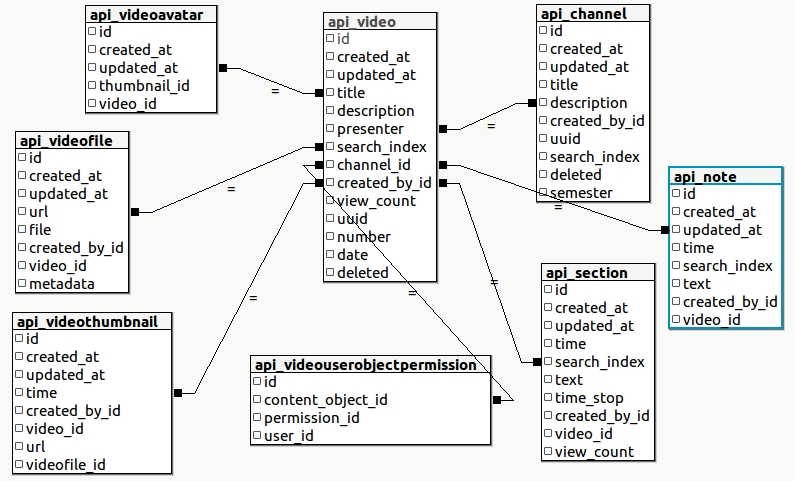
\includegraphics[width=1\textwidth]{images/db.jpg}
  \caption{Структура базы данных для хранения видео\label{db}}
\end{figure}


Данная структура позволяет хранить описание этих объектов такое как: тип объекта,
набор его полей, с указанием типа полей, а так же заданием особого поведения для
некоторых полей объекта.

Основные сущности были выделены в отдельные таблицы, структура базы данных включает
все необходимые элементы для эффективного хранения и представления данных приложения,
при необходимости она может быть легко расширена.

\subsection{Разграничение прав доступа на объекты}

Приложение реализует проверку прав на объект, а не на всю
модель (object-level permissions) c помощью django-guardian. Начиная с Django 1.2 бэкенд
аутентификации поддерживает проверку прав на объект, но это не реализовано в самом Django.
django-guardian успешно заполняет этот пробел. Пример описания прав доступа к видеообъекту
приведен в листинге ~\ref{lst:permissions}:

\FloatBarrier

\begin{lstlisting}[caption={Пример описания прав доступа}, label=lst:permissions]
class ChannelVideoPermissionContext(dict):
  def __init__(self, user_permission_context):
    self._pc = user_permission_context
    super(ChannelVideoPermissionContext, self)
      .__init__(**{
      'view': self._has(
        'view_video',
        'play_video',
        'view annotation_video',
        'annotate_video',
        'change annotation_video',
        'change_video'
      ),
      'watch': self._has(
        'play_video',
        'view annotation_video',
        'annotate_video',
        'change annotation_video',
        'change_video'
      )
    })
\end{lstlisting}

\subsection{Разработка пользовательского интерфейса}

В ходе анализа существующих решений, а также изучения бизнес требований предъявляемых к системе,
был разработан базовый набор модулей, необходимых для управления платформой видеолекций.
\begin{figure}
  \centering
  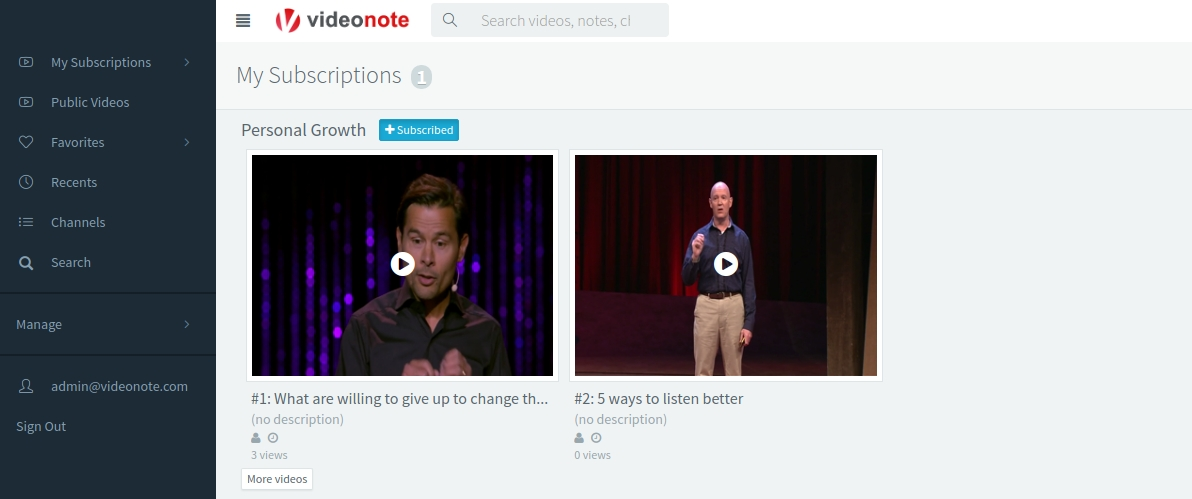
\includegraphics[width=1\textwidth]{images/user-interface.jpg}
  \caption{Список лекций\label{user-interface}}
\end{figure}

На рисунке \ref{user-interface} представлен фрагмент пользовательского интерфейса приложения.
Видео разбиты по тематическим каналам. Есть возможно оформить подписку на канал - видео с этих
каналов будут отображаться в разделе "My Subscriptions".

\begin{figure}
  \centering
  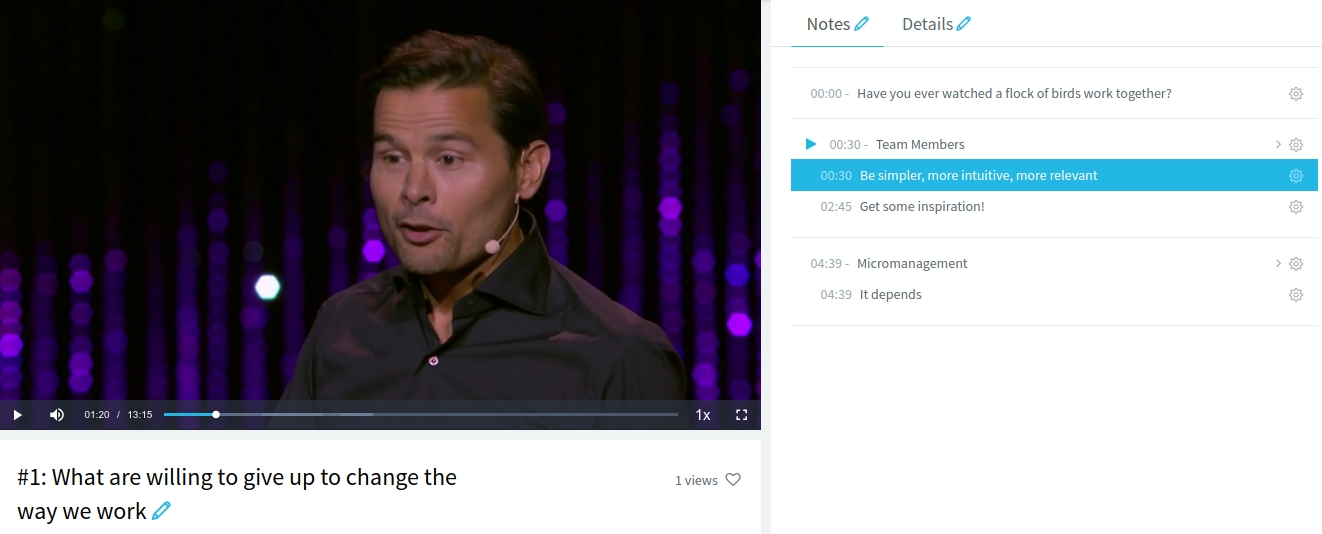
\includegraphics[width=1\textwidth]{images/annotations.jpg}
  \caption{Аннотации при просмотре видео}\label{annotations}
\end{figure}

На рисунке \ref{annotations} показана страница просмотра лекции. В блоке с аннотациями
выводятся заметки, сгруппированные в секции, привязанные к текущему таймфрему видео.
При клике на секцию происходит переход к соответсвующему фрагменту видео. Здесь же, при просмотре
видео, есть возможность добавления/редактирования аннотаций лектором.

На рисунке \ref{search} отображен блок поиска. Поиск осуществляется не только по названиям лекций,
но и по аннотоациям к видео: секциям и заметкам, а также по каналам. При клике приосходит переход
сразу к каналу, к видео либо к нужному фрагменту видео.

\begin{figure}
  \centering
  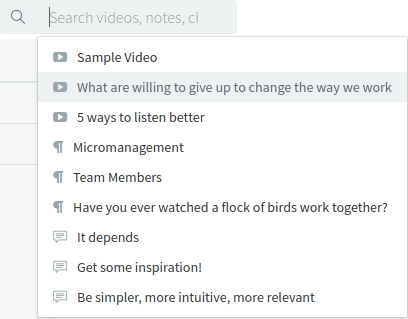
\includegraphics[width=0.7\textwidth]{images/search.jpg}
  \caption{Поиск}\label{search}
\end{figure}

Для видеофайла можно настроить доступ. Видео может быть доступно для всех или только для
определенных групп пользователей. Дополнительно можно настроить кто может редактировать и
аннотировать видео. На рисунке \ref{permissions} показаны настройки доступа к видео. Можно
выбрать отдельных пользователей либо целые группы и настроить для них необходимые разрешения.

\begin{figure}
  \centering
  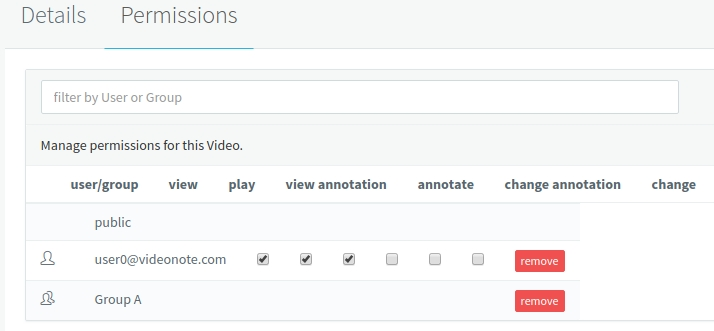
\includegraphics[width=0.9\textwidth]{images/permissions.jpg}
  \caption{Настройка доступов к видеофайлу}\label{permissions}
\end{figure}
